\section{Redes Adversárias Geradoras}
\label{sec:gan}
\index{GAN}
\index{RAG}
\index{Redes Adversárias Geradoras}

Uma forma relativamente nova na indústria para gerar dados, é a utilização das \textit{redes geradoras adversárias}\index{GAN}. O conceito foi introduzido em 2014 por \citeonline{goodfellow_generative_2014}. As redes geradoras utilizam o princípio da competição para produzir os resultados e para disso, utiliza (pelo menos na arquitetura inicial proposta) duas redes neurais, competindo entre si para gerar quaisquer forma de dados que sejam aplicáveis à esse tipo de modelo.

O modelo consiste de duas redes neurais denominadas \textit{geradora} ($G(x)$) e \textit{discriminadora} ($D(y)$). A geradora, como o próprio nome diz gera o dado em questão: imagens, texto, música entre outros \cite{c_han_gan-based_2018, xu_diversity-promoting_2018, oza_progressive_2019}. 

A rede discriminadora, tem uma função simples: validar o que a geradora produz. Esta rede detecta se o que foi produzido pela geradora é falso ou não. Seja o problema de se implementar uma RAG (sigla para redes geradoras adversárias) capaz de gerar imagens de pôr do sol. A rede discriminadora será treinada para identificar o que é e o que não é uma imagem de pôr do sol enquanto a rede geradora será treinada para a enganar. Taí a competição: enquanto a rede \textit{D} fica melhor em detectar se uma imagem é falsa ou não, a rede \textit{G} fica melhor em enganar a rede \textit{D} a achar se que o que ela está produzindo, é uma imagem verdadeira de pôr do sol.

\begin{figure}[H]
    \centering
    \caption{Diagrama de uma RAG.}
    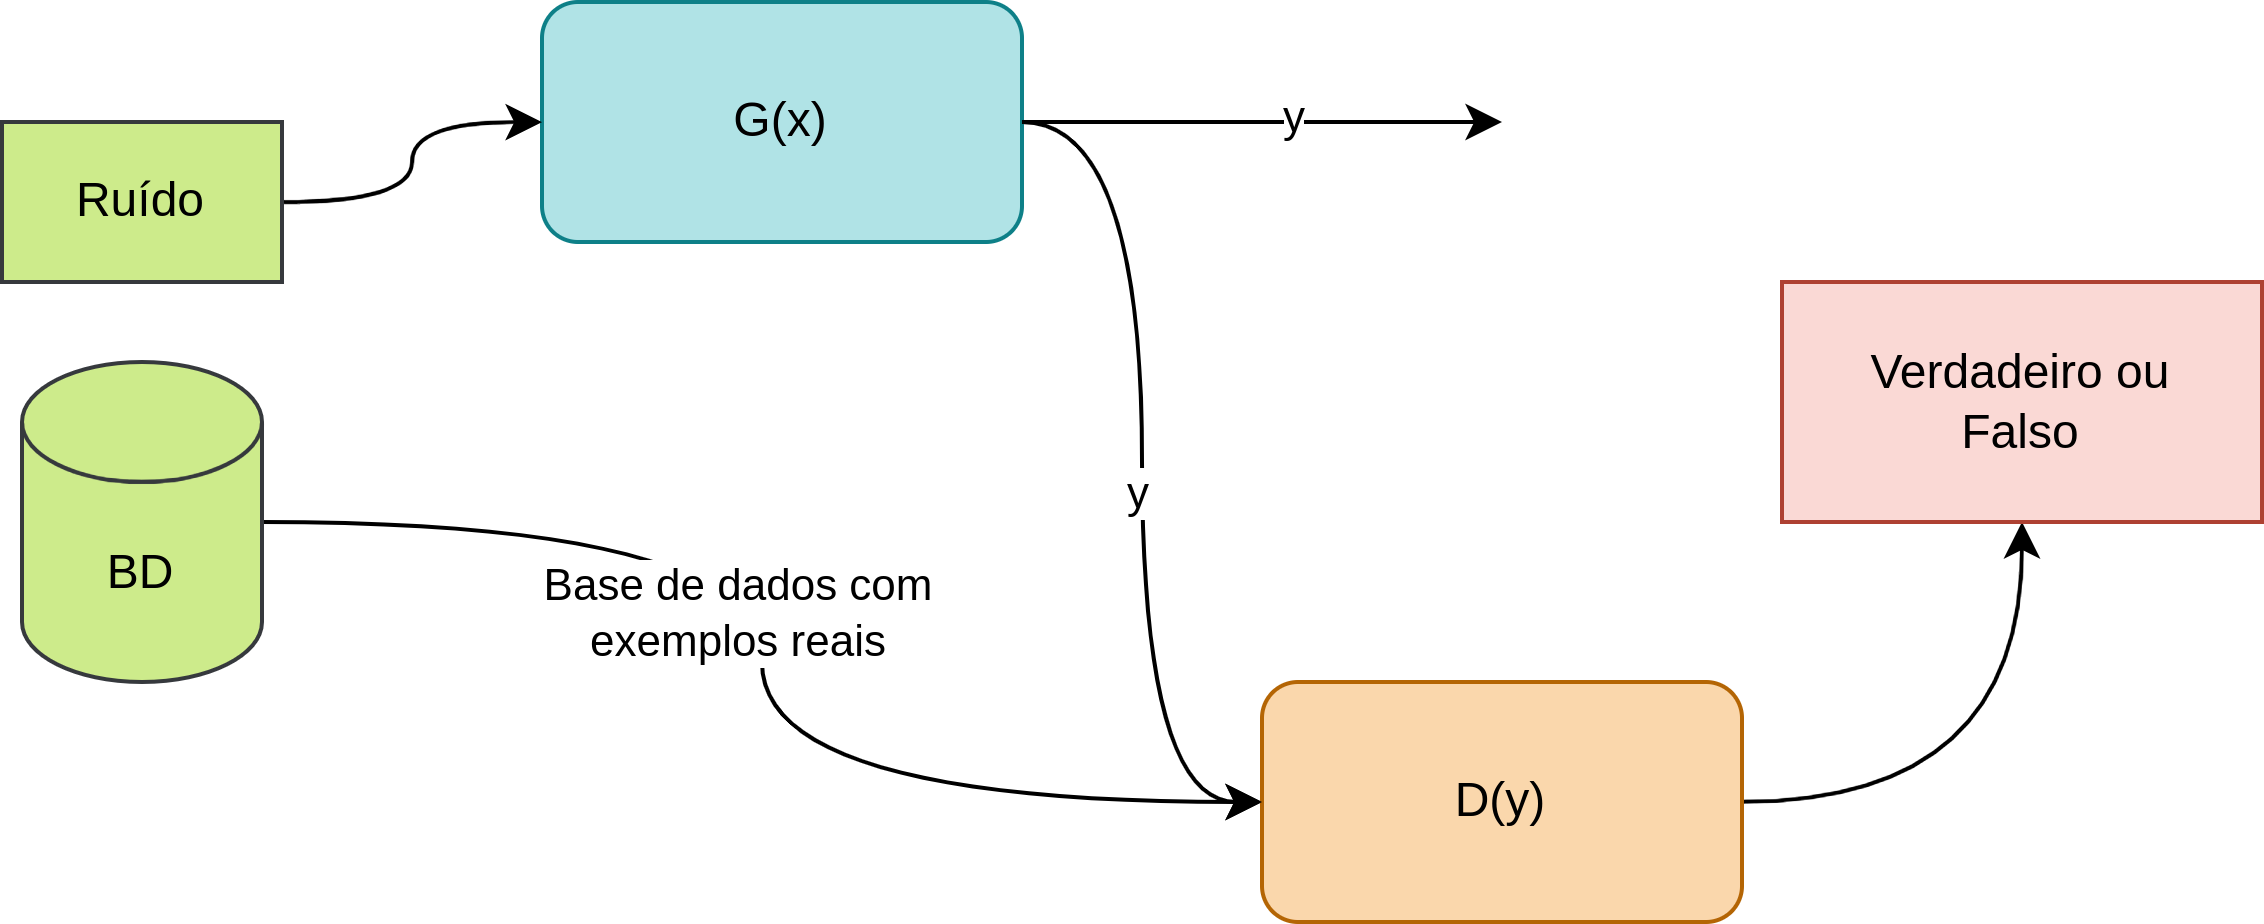
\includegraphics[width=11cm]{fig/GAN_2.png}
    \legend{Fonte: autor, baseado em \cite{gulli_deep_2019, zhang_dive_2021, moreira_geracao_2019}.}
    \label{fig:fig7}
\end{figure}

De acordo com a imagem \ref{fig:fig7}, a saída da rede geradora alimenta a rede discriminadora, assim como dados reais também entram nesta. Estes são utilizados para treiná-la a diferenciar com cada vez mais precisão um dado falso de um verdadeiro (ou, gerado de real). No caso de super-resolução de imagens, estes dados são em forma de imagens. A geradora é treinada para converter ruído em imagens. Imagens estas, que por sua vez sejam capazes de enganar a discriminadora a classificar se a imagem gerada é uma imagem verdadeira. Uma vez que as imagens artificialmente geradas são capazes de se passarem por imagens verdadeiras (entenda \textit{se passarem por imagens verdadeiras} como serem identificadas como imagens reais), a rede geradora estará produzindo imagens semelhantes às imagens nas quais a rede discriminadora foi treinada para identificar. O termo "semelhante", utilizado da forma como foi utilizado, pode ser subjetivo. Para os olhos humanos, é natural e intuitivo avaliar se duas imagens são parecidas ou não. No contexto de modelos de redes neurais, a semelhança é avaliada até onde o modelo consegue capturar e reproduzir padrões.

\subsection{SRGAN}
\index{GAN} 
\index{SRGAN} 
\index{Super Resolution Generative Adversarial Networks}

SRGAN é a arquitetura de GAN proposta para fazer super-resolução de imagens. Ela utiliza duas redes (discriminadora e geradora), montadas individualmente em arquiteturas específicas para obter o máximo das redes na super-resolução. O diagrama \ref{fig:fig8} abaixo mostra como a rede é organizada. O nome das camadas são dados por k<x>n<y>s<z>, onde \textit{x} é o tamanho do kernel, \textit{y} é o número de \textit{feature maps} (i.e. o tamanho da saída da camada convolucional) e \textit{s} é a sigla para \textit{stride}, que representa o passo que a janela de pooling vai se deslocar em cada iteração (e.g. com \textit{s=1}, a janela de \textit{pooling} vai se deslocar de pixel a pixel) 

\begin{figure}[H]
    \centering
    \caption{Diagrama da SRGAN.}
    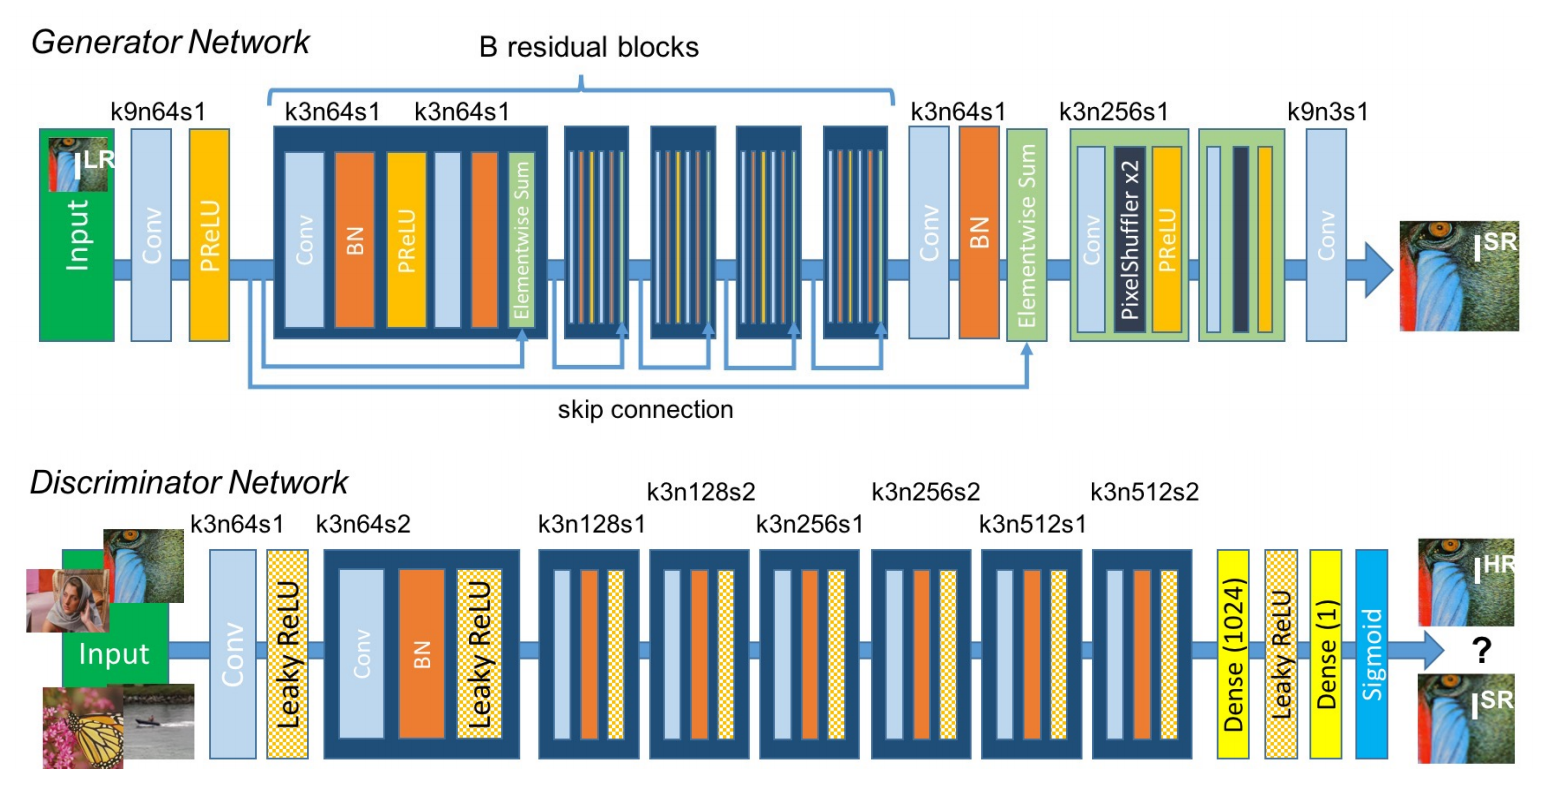
\includegraphics[width=11cm]{fig/SRGAN.png}
    \legend{Fonte: \cite{ledig_photo-realistic_2017}}
    \label{fig:fig8}
\end{figure}

Neste modelo, a discriminadora é treinada para avaliar se a imagem é uma imagem original de alta resolução ou uma imagem super-resolvida artificialmente \cite{ledig_photo-realistic_2017} enquanto a geradora (essa parte difere um pouco da arquitetura original proposta por \citeonline{goodfellow_generative_2014}) é treinada para processar uma imagem de baixa resolução (anteriormente, no lugar da imagem em baixa resolução, a entrada era ruído), processá-la, e obter uma imagem de maior resolução na saída.

\subsection{ESRGAN}
\index{GAN} 
\index{ESRGAN} 
\index{Enhanced Super Resolution Generative Adversarial Networks}

A SRGAN, obteve grande desempenho em relação aos outros modelos testados porém, \citeonline{wang_esrgan_2018} detectou alguns pontos na arquitetura que podem ser otimizados. Perceba, que na figura \ref{fig:fig8}, a rede geradora é formada por um conjunto de blocos básicos (\textit{B residual blocks}). Esses blocos, internamente são formados por uma série de camadas e entre elas temos uma camada representada pela cor laranja, identificada como BN. Vide figura \ref{fig:fig12}.

\begin{figure}[H]
    \centering
    \caption{Diagrama do bloco básico da SRGAN.}
    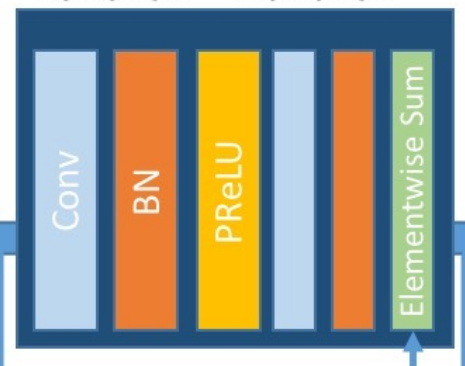
\includegraphics[width=7cm]{fig/basic-block.png}
    \legend{Fonte: \cite{ledig_photo-realistic_2017}}
    \label{fig:fig12}
\end{figure}

A camada \textit{BN} da imagem \ref{fig:fig12} performa uma normalização na saída da camada anterior chamada \textit{Batch Normalization}. Esta normalização reduz alguns problemas existentes no treinamento de redes neurais, performando uma normalização não a nível de amostra, mas a nível de \textit{batches}, que são um conjunto de dados treinados em sequência numa rede. De acordo com \citeonline{wang_esrgan_2018}, esta normalização não é eficiente quando o modelo está lidando com otimização de dados utilizando relação sinal-ruído. Para tal, \citeonline{wang_esrgan_2018} propõe um novo modelo de bloco básico e um novo modelo de rede discriminadora. A figura \ref{fig:fig13} ilustra o novo bloco básico proposto, que elimina completamente as camadas de normalização de \textit{batch}.
 
\begin{figure}[H]
    \centering
    \caption{Diagrama do novo bloco básico da ESRGAN.}
    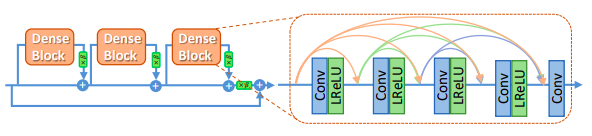
\includegraphics[width=11cm]{fig/new-basic-block.png}
    \legend{Fonte: \cite{wang_esrgan_2018}}
    \label{fig:fig13}
\end{figure} 
